\section{Auswertung}

Die Temperatur wurde nicht direkt gemessen, sondern es wurde ein Widerstandstermometer verwendet.
Die gemessenen Widerstände können mithilfe der \autoref{fig:abb3} in eine Temperatur umgerechnet werden.
\begin{figure}[H]
  \centering
  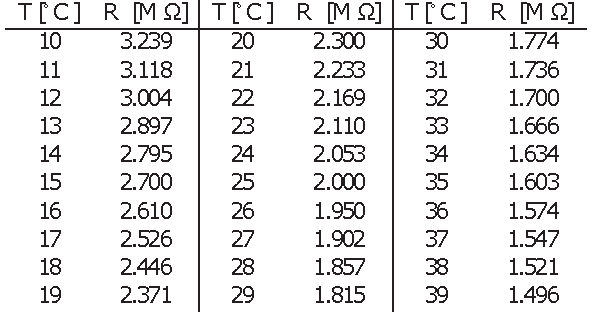
\includegraphics{figures/Temperatur.pdf}
  \caption{Temperatur der Luft bei verschiedenen Widerständen \cite{ap12}\, .} 
  \label{fig:abb3}
\end{figure}
Die Viskusität von Luft kann durch die \autoref{fig:viskositaet} bestimmt werden.
\begin{figure}[H]
  \centering
  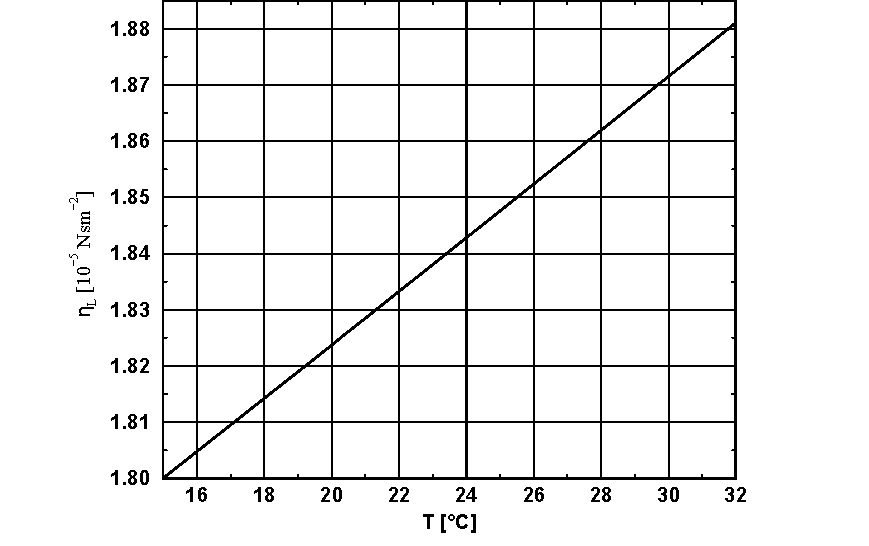
\includegraphics{figures/Viskositaet.pdf}
  \caption{Die Viskosität von Luft bei verschiedenen Temperaturen  \cite{ap12}\, .} 
  \label{fig:viskositaet}
\end{figure}



Um die Ladung der Öltröpfchen zu ermitteln, wurden Messungen bei fünf verschiedenen Spannungen für jeweils fünf Tröpfchen durchgeführt.
Alle Zeiten wurden für eine Strecke von $s = 5 \, \unit{\milli\meter}$ gemessen.
\begin{table}[H]
    \caption{Messdaten der Öltröpfchen für verschiedene Spannungen}
    \label{tab:v_werte}
    \centering
    \begin{minipage}[t]{1\textwidth}
        \small
        \subcaption{Daten für $U=\qty{157}{\volt}$}
        \label{stab:v157}
        \begin{table}[H]
            \centering
            \begin{tabular}{S S S S S}
              \toprule
                {$R \mathbin{/} \unit{\mega\ohm} $}& {$T \, \text{in} °C $} & {$\eta \, \text{in} 10^{-5} \unit{\newton}\mathbin{/} \unit{\second\meter}^2$} & {$ t_{ab} \mathbin{/} \unit{\second}$} & {$ t_{auf} \mathbin{/} \unit{\second}$}\\
              \midrule
              
              \bottomrule
            \end{tabular}
          \end{table}
        
    \end{minipage}\qquad
    \begin{minipage}[t]{1\textwidth}
        \small
        \subcaption{Daten für $U=\qty{175}{\volt}$}
        \label{stab:v175}
        \begin{table}[H]
            \centering
            \begin{tabular}{S S S S S}
              \toprule
                {$R \mathbin{/} \unit{\mega\ohm} $} & {$T \, \text{in} °C $} & {$\eta \, \text{in} 10^{-5} \unit{\newton}\mathbin{/} \unit{\second\meter}^2$}&{$ t_{ab} \mathbin{/} \unit{\second}$} & {$ t_{auf} \mathbin{/} \unit{\second}$}\\
              \midrule
              
              \bottomrule
            \end{tabular}
          \end{table}
        
    \end{minipage}\qquad
    \begin{minipage}[t]{1\textwidth}
        \small
        \subcaption{Daten für $U=\qty{200}{\volt}$}
        \label{stab:v200}
        \begin{table}[H]
            \centering
            \begin{tabular}{S S S S S}
              \toprule
                {$R \mathbin{/} \unit{\mega\ohm} $} & {$T \, \text{in} °C $} & {$\eta \, \text{in} 10^{-5} \unit{\newton}\mathbin{/} \unit{\second\meter}^2$}&{$ t_{ab} \mathbin{/} \unit{\second}$} & {$ t_{auf} \mathbin{/} \unit{\second}$}\\
              \midrule
              
              \bottomrule
            \end{tabular}
          \end{table}
        
    \end{minipage}\qquad
    \begin{minipage}[t]{1\textwidth}
        \small
        \subcaption{Daten für $U=\qty{225}{\volt}$}
        \label{stab:v225}
        \begin{table}[H]
            \centering
            \begin{tabular}{S S S S S}
              \toprule
                {$R \mathbin{/} \unit{\mega\ohm} $} & {$T \, \text{in} °C $} & {$\eta \, \text{in} 10^{-5} \unit{\newton}\mathbin{/} \unit{\second\meter}^2$}&{$ t_{ab} \mathbin{/} \unit{\second}$} & {$ t_{auf} \mathbin{/} \unit{\second}$}\\
              \midrule
              
              \bottomrule
            \end{tabular}
          \end{table}
        
    \end{minipage}\qquad
    \begin{minipage}[t]{1\textwidth}
        \small
        \subcaption{Daten für $U=\qty{250}{\volt}$}
        \label{stab:v250}
        \begin{table}[H]
            \centering
            \begin{tabular}{S S S S S}
              \toprule
                {$R \mathbin{/} \unit{\mega\ohm} $} & {$T \, \text{in} °C $} & {$\eta \, \text{in} 10^{-5} \unit{\newton}\mathbin{/} \unit{\second\meter}^2$}&{$ t_{ab} \mathbin{/} \unit{\second}$} & {$ t_{auf} \mathbin{/} \unit{\second}$}\\
              \midrule
              
              \bottomrule
            \end{tabular}
          \end{table}
    \end{minipage}
\end{table}
Mit dem Zeit-Weg-Gesetzt \eqref{eq:Zeitweg}
\begin{equation*}
  v = \dfrac{s}{t}
  \label{eq:Zeitweg}
\end{equation*}

wird die Geschwindigkeit der von jedem einzelnen Tröpfchen bestimmt.
Die Geschwindigkeit sind in \autoref{tab:geschw} aufgetragen.
\begin{table}[H]
  \caption{Geschwindigkeiten der Öltröpfchen für verschiedene Spannungen}
  \label{tab:geschw}
  \centering
  \begin{minipage}[t]{0.45\textwidth}
      \small
      \subcaption{Daten für $U=\qty{157}{\volt}$}
      \label{stab:v157}
      \begin{table}[H]
          \centering
          \begin{tabular}{S S S}
            \toprule
              {Nr}& {$ v_{ab} \mathbin{/} \dfrac{\unit{\micro\meter}}{\unit{\second}}$}&{$ v_{auf} \mathbin{/} \dfrac{\unit{\micro\meter}}{\unit{\second}}$}\\
            \midrule
            
            \bottomrule
          \end{tabular}
        \end{table}
      
  \end{minipage}\qquad
  \begin{minipage}[t]{0.45\textwidth}
      \small
      \subcaption{Daten für $U=\qty{175}{\volt}$}
      \label{stab:v175}
      \begin{table}[H]
          \centering
          \begin{tabular}{S S S}
            \toprule
            {Nr}& {$ v_{ab} \mathbin{/} \dfrac{\unit{\micro\meter}}{\unit{\second}}$}&{$ v_{auf} \mathbin{/} \dfrac{\unit{\micro\meter}}{\unit{\second}}$}\\
            \midrule
            
            \bottomrule
          \end{tabular}
        \end{table}
      
  \end{minipage}\qquad
  \begin{minipage}[t]{0.45\textwidth}
      \small
      \subcaption{Daten für $U=\qty{200}{\volt}$}
      \label{stab:v200}
      \begin{table}[H]
          \centering
          \begin{tabular}{S S S}
            \toprule
            {Nr}& {$ v_{ab} \mathbin{/} \dfrac{\unit{\micro\meter}}{\unit{\second}}$}&{$ v_{auf} \mathbin{/} \dfrac{\unit{\micro\meter}}{\unit{\second}}$}\\
            \midrule
            
            \bottomrule
          \end{tabular}
        \end{table}
      
  \end{minipage}\qquad
  \begin{minipage}[t]{0.45\textwidth}
      \small
      \subcaption{Daten für $U=\qty{225}{\volt}$}
      \label{stab:v225}
      \begin{table}[H]
          \centering
          \begin{tabular}{S S S}
            \toprule
              {Nr}& {$ v_{ab} \mathbin{/} \dfrac{\unit{\micro\meter}}{\unit{\second}}$}&{$ v_{auf} \mathbin{/} \dfrac{\unit{\micro\meter}}{\unit{\second}}$}\\
            \midrule
            
            \bottomrule
          \end{tabular}
        \end{table}
      
  \end{minipage}\qquad
  \begin{minipage}[t]{0.45\textwidth}
      \small
      \subcaption{Daten für $U=\qty{250}{\volt}$}
      \label{stab:v250}
      \begin{table}[H]
          \centering
          \begin{tabular}{S S S}
            \toprule
              {Nr}& {$ v_{ab} \mathbin{/} \dfrac{\unit{\micro\meter}}{\unit{\second}}$}&{$ v_{auf} \mathbin{/} \dfrac{\unit{\micro\meter}}{\unit{\second}}$}\\
            \midrule
            
            \bottomrule
          \end{tabular}
        \end{table}
  \end{minipage}
\end{table}

Die Ladungen der Tröpfchen sind in \autoref{tab:Ladungen} aufgetragen. Dazu muss zunächst die effektive Viskosität mit \eqref{eq:Veff}, der Radius der Tröpfchen \eqref{eq:rmitEfled} und die korrigierte Ladung \eqref{eq:qKorr} berechnet werden.

\begin{table}[H]
  \centering
  \caption{Messreihe für senkrechte Polarisation.}
  \label{tab:Ladungen}
  \begin{tabular}{S S}
    \toprule
      {$\text{Nr}$} & {$q \, \text{in} \mathbin{/} \unit{\coulomb}$}\\
    \midrule

    \bottomrule
  \end{tabular}
\end{table}

Es ist unrealistisch, dass alle Ladungen ein ganzzahliges vielfachen von einem einzelnen Wert sind, deswegen wird nach dem kleinsten gemeinsammen Teilcher gesucht, bei dem die übrigbleibende Differenz unter $1 \cdot 10^{-19}$ liegt, da die Elementarladung in dieser Größenordnung vermutet wird.
Mit dieser Methode wird eine Ladund von 
\begin{equation}
%  e_0 = \qty{wert(unsicherheit)e-19} \,\unit{\coulomb}
  \label{eq:egemessen}
\end{equation}
berechnet.
Daraus kann über die Faraday-Konstante $ F = 96485,33212... \dfrac{\unit{\coulomb}}{\text{mol}}$ \cite{go02} mit der Gleichung 
\begin{equation*}
  N_\text{A} = \dfrac{F}{e_0}
  \label{eq:egemessen}
\end{equation*}
die Avogadro-Konstante bestimmt werden, welche 

\begin{equation*}
%  N_\text{A} = \qty{wert(unsicherheit)e23} \, \dfrac{1}{mol}
  \label{eq:egemessen}
\end{equation*}
als Wert hat.